%!xelatex = 'xelatex --halt-on-error %O %S'

\documentclass{thuemp}
\begin{document}

% 标题,作者
\emptitle{巨磁电阻效应及其应用}
\empauthor{王驰}{王合英}

% 奇数页页眉 % 请在这里写出第一作者以及论文题目
\fancyhead[CO]{{\footnotesize 王驰: 巨磁电阻效应及其应用}}


%%%%%%%%%%%%%%%%%%%%%%%%%%%%%%%%%%%%%%%%%%%%%%%%%%%%%%%%%%%%%%%%
% 关键词 摘要 首页脚注
%%%%%%%%关键词
\Keyword{巨磁电阻效应,磁传感器,磁电转换,自旋电子学,纳米材料}
\twocolumn[
\begin{@twocolumnfalse}
\maketitle

%%%%%%%%摘要
\begin{empAbstract}
本实验利用 ZKY-JCZ 型巨磁电阻效应实验仪,系统研究了多层薄膜 GMR 器件的磁阻特性及其应用。通过直接测量 GMR 元件的电阻-磁场曲线,观察到显著的磁阻效应($\Delta R/R \approx 13\%$)和磁滞现象;测量了模拟传感器的线性磁电转换特性(灵敏度 $0.236\ \mathrm{mV/mT}$)和开关传感器的阈值特性(开关场 $\pm 0.4\ \mathrm{mT}$);探究了偏置磁场对电流测量的影响,发现适当偏置可将线性度提升至 $r^2 > 0.999$;利用梯度传感器实现了角位移检测(周期 $24^\circ$),并通过磁读写组件验证了二进制数据存储。实验表明,GMR 效应在传感器技术和信息存储中具有重要应用价值。
\end{empAbstract}

%%%%%%%%英文标题、作者、摘要、关键词
\emptitleEn{Experiments of Modern Physics in Tsinghua University}
\empauthorEn{Chi Wang}{Heying Wang}
\KeywordEn{keyword1, keyword2, keyword3, keyword4, keyword5}

\begin{empAbstractEn}
This experiment systematically investigated the magnetoresistance characteristics and applications of multilayer GMR devices using a ZKY-JCZ giant magnetoresistance effect instrument. Direct measurement of resistance-magnetic field curves revealed significant magnetoresistance ($\Delta R/R \approx 13\%$) and hysteresis. The analog sensor exhibited linear magnetoelectric conversion (sensitivity $0.236\ \mathrm{mV/mT}$), while the switch sensor showed threshold characteristics (switching field $\pm 0.4\ \mathrm{mT}$). Current measurement experiments demonstrated that appropriate bias magnetic fields improve linearity ($r^2 > 0.999$). Angular displacement detection was achieved using a gradient sensor ($24^\circ$ period), and binary data storage was verified via magnetic read/write components. The results confirm the importance of GMR effects in sensor technology and information storage.
\end{empAbstractEn}

%%%%%%%%首页角注,依次为实验时间、报告时间、学号、email
\empfirstfoot{2025-04-20}{2025-05-07}{2022012259}{chi-wang22@mails.tsinghua.edu.cn}
\end{@twocolumnfalse}
]
%%%%%%%%!首页角注可能与正文重叠,请通过调整正文中第一页的\enlargethispage{-3.3cm}位置手动校准正文底部位置:
%%%%%%%%%%%%%%%%%%%%%%%%%%%%%%%%%%%%%%%%%%%%%%%%%%%%%%%%%%%%%%%%
%  正文由此开始
\wuhao 
%  分栏开始

\section{引言}
\enlargethispage{-3.3cm}
巨磁电阻效应(Giant Magnetoresistance, GMR)是铁磁/非磁多层膜中电阻随外磁场显著变化的现象,由 Fert 和 Grünberg 于 1988 年独立发现 \cite{BAIBICH19882472,BINASCH19894828},两人因此获 2007 年诺贝尔物理学奖。该效应源于自旋相关散射,遵循双电流模型和 RKKY 交换作用理论 \cite{PARKIN19902304},其核心特征是相邻铁磁层的磁矩从反平行(高阻)转向平行排列(低阻)。GMR 器件具有灵敏度高、响应快、抗干扰强等优势,已广泛应用于硬盘磁头、磁传感器和随机存储器等领域 \cite{王合英2008磁控溅射镀膜过程中非均匀磁场中电子的运动}。

本实验旨在通过七组测量系统探究 GMR 效应:1) 直接测量磁阻特性曲线,2) 分析模拟传感器磁电转换特性,3) 研究数字传感器开关行为,4) 实现非接触式电流测量,5) 构建角位移传感器,6) 验证磁记录原理,7) 探索自旋阀磁电阻。通过定量分析磁滞、线性度、灵敏度等参数,为磁电子器件的设计与优化提供实验依据。

\section{实验内容}

在本实验中,我们使用ZKY-JCZ型巨磁电阻效应及应用实验仪,对实验仪内附的各GMR器件进行实验。

在 GMR 模拟传感器中,四个近似相同的多层薄膜 GMR 电阻构成一个电桥结构(如图 \ref{fig:gmr_bridge} 所示)。若 4 个 GMR 电阻对磁场的响应完全相同,电桥平衡,电压输出端将不会有信号电压输出。

\begin{figure}[H]
    \centering
    \begin{circuitikz}[scale=0.6, transform shape, european resistors]
    \tikzstyle{every node}=[font=\LARGE]
    
    % 电桥主体结构
    \draw (3.75,12.25) to[european resistor, l=$R_1$] (7.5,12.25);
    \node at (7.5,12.25) [circ] {};
    \draw (7.5,12.25) to[european resistor, l=$R_3$] (11.25,12.25);
    
    % 在电桥中央直接标注U_OUT
    \node at (7.5,9.75) {$U_{OUT}$}; % 直接在中央位置添加标注
    \draw (7.5,12.25) to[short, -o] (7.5,11.0) node[below] {+};
    \draw (7.5,7.25) to[short, -o] (7.5,8.5) node[above] {-};
    \draw (7.5,7.25) to[european resistor, l_=$R_2$] (3.75,7.25);
    \draw (7.5,7.25) to[european resistor, l=$R_4$] (11.25,7.25); % R_4标签移到上方
    
    % 输入电压
    \draw (2.5,9.75) to[short, -o] (2.5,4.75) node[below] {$U_{IN+}$};
    \draw (12.5,9.75) to[short, -o] (12.5,4.75) node[below] {GND};
    
    % 连接线
    \node at (3.75,9.75) [circ] {};
    \node at (11.25,9.75) [circ] {};
    \draw (3.75,12.25) to[short] (3.75,7.25);
    \draw (11.25,12.25) to[short] (11.25,7.25);
    \draw (12.5,9.75) to[short] (11.25,9.75);
    \draw (3.75,9.75) to[short] (2.5,9.75);
    
    % 磁屏蔽层(坡莫合金)- 标注移到框外
    \draw [dashed] (8,13.5) rectangle (10.75,11.5);
    \node [above] at (9.375,13.5) {屏蔽层}; % 移到框的上方外部
    
    \draw [dashed] (4.25,8.5) rectangle (7,6.5);
    \node [below] at (5.625,6.5) {屏蔽层}; % 移到框的下方外部
    
    \end{circuitikz}
    \caption{GMR模拟传感器电桥结构}
    \label{fig:gmr_bridge}
\end{figure}

\begin{figure}[H]
\centering
\begin{circuitikz}[scale=0.8, transform shape]
  % 绘制GMR元件(居中)
  \draw (0,0) rectangle (2,1) node[pos=0.5] {GMR};
  
  % 电流引线(对称等长)
  \draw (0,0.5) to[short, -o] (-2,0.5) node[left] {$I_+$};
  \draw (2,0.5) to[short, -o] (4,0.5) node[right] {$I_-$};
  
  % 电压引线(缩短长度,对称布局)
  \draw (0.5,1) to[short] (0.5,1.5) to[short, -o] (0.5,3) node[above] {$V_+$};
  \draw (1.5,1) to[short] (1.5,1.5) to[short, -o] (1.5,3) node[above] {$V_-$};
  
\end{circuitikz}
\caption{四端接线法测量原理}
\label{fig:four_terminal}
\end{figure}
值得注意的是,实验中所使用的GMR元件自身阻值较小,为消除引线电阻和接触电阻对测量结果的干扰,各个传感器中均采用四端接线法进行测量(见图\ref{fig:four_terminal})。该方法通过分离电流驱动与电压检测路径:电流端子($I_+$, $I_-$)向元件注入恒定电流,电压端子($V_+$, $V_-$)在元件内部直接测量电势差。由于电压测量回路输入阻抗极高(通常>10 MΩ),流经电压引线的电流可忽略不计,从而有效规避了引线电阻、接触电阻及连接点温漂引入的误差。


\subsection{磁阻特性曲线测量}

在本部分实验中,不利用GMR模拟传感器的电桥结构,而直接使用伏安法测量$R_1$和$R_2$的电阻值随外加磁场的变化。


实验仪选择“磁电阻测量模式”,此时$R_3$和$R_4$被短接,$R_1$和$R_2$直接并联。外接SB119型恒压源以及电流表$\mathrm{A_1}$,形成伏安法测量电阻电路。使用一个线圈密度为$n=24000~ \mathrm{m^{-1}}$的螺线管施加磁场,将GMR传感器置于螺线管中部;设定恒压源输出电压为$4~\mathrm{V}$,励磁电流$I_m$取$-99.7 ~ \mathrm{mA}$至$100.5 ~ \mathrm{mA}$的范围内一系列值,先后单向增大和减小外磁场,过程中记录电流表$\mathrm{A_1}$示数$I_R$,间接得到电阻值随外加磁场变化情况。


对各个实验数据点,利用螺线管磁感应强度公式$B=\mu_0 n I_m$以及欧姆定律,计算得到磁感应强度以及相对应的电阻值,据此可绘制磁阻特性曲线。

\subsection{GMR模拟传感器的磁电转换特性测量}

在本部分实验中,实验仪选择“传感器测量”模式,设定恒压源输出电压为$4~\mathrm{V}$,此时$R_1, R_2, R_3, R_4$构成电桥结构;于“模拟信号输出”端口接入电压表$\mathrm{V_1}$,形成电桥测量电路。使用与2.1节中相同的线圈施加磁场,GMR传感器保持在螺线管中部,在励磁电流$I_m$取$-101.9 ~ \mathrm{mA}$至$100.5 ~ \mathrm{mA}$的范围内,先后单向增大和减小外磁场,过程中记录电压表示数$U_s$,进而得到输出电压与外加磁场的关系。

对各个实验数据点,同样利用螺线管磁感应强度公式$B=\mu_0 n I_m$,计算得到磁感应强度,绘制磁电转换特性曲线。

\subsection{GMR开关(数字)传感器的磁电转换特性测量}

在本部分实验中,于实验仪“开关信号输出”端口接入电压表$\mathrm{V_1}$,此时GMR电桥输出电压经比较电路以及放大电路处理后,形成电压表读取到的开关信号。在这里,比较电路以及放大电路使得当GMR开关传感器的输出电压大于设定的阈值时,电压表$\mathrm{V_1}$显示“高电平”,否则显示“低电平”。

在本实验中,在励磁电流$I_m$取$-40 ~ \mathrm{mA}$至$40 ~ \mathrm{mA}$的范围内,先后单向增大和减小外磁场,过程中记录高低电平对应的电压表示数,以及发生高低电平之间发生跃变对应的临界励磁电流。同样从临界励磁电流得到临界磁感应强度,给出开关传感器的磁电转换特性曲线。

\subsection{使用GMR模拟传感器测量电流}

本部分实验探究使用GMR模拟传感器测量电流,并通过对照实验探究偏置磁场对测量结果的影响。在本部分实验中,利用实验仪以及电流测量组件,使用一可调电流源为导线提供电流$I_s$,GMR模拟传感器固定在导线中段旁侧,使用一块永磁体(可活动)提供偏置磁场。

先后在有低磁偏置和适当磁偏置条件下,在导线上沿两个方向通电流,并在$I_s$取$-300~300\mathrm{mA}$范围内单向增减,分别测量记录输出电压$U_s$,绘制$U_s - I_s$关系曲线图,并对不同磁偏置条件测量结果对比。

\subsection{GMR梯度传感器的特性及应用}

本部分实验对GMR梯度传感器特性以及应用展开探究。通过将GMR电桥两对对角位置电阻分别置于集成电路两端,并且不添加磁屏蔽,即可制成GMR梯度传感器。若在均匀磁场中,4个桥臂电阻始终相等,电桥输出电压恒为0。但若置于具有一定梯度的外磁场中,各个GMR元件的电阻变化不相同步,电桥平衡破坏,输出电压即可反映传感器附近磁场大小的梯度。

利用GMR梯度传感器的上述特性,可制成角位移传感器:在角位移测量组件内,GMR梯度传感器一侧安装有永磁体,另一侧为铁磁性材料制成的齿轮。伴随齿轮转动,GMR梯度传感器所处位置的磁场梯度状况发生周期性变化,且每一周期恰对应移动过一齿。据此周期性变化,即可测量角位移以及旋转部件转速。

在本部分实验中,先后将齿轮转过$0^\circ~48^\circ$之间的一系列角度,记录GMR电桥输出电压,作图,可得到齿轮位移与输出电压关系。

\subsection{磁记录与读出}

本部分实验探究使用磁读写组件,进行磁性记录材料中中信息写入以及使用自旋阀器件进行信息读出。磁读写组件中集成了一个具有铁芯的线圈作为写入单元(写磁头),和一个自旋阀巨磁阻元件作为读出单元(读磁头)。

在本实验中,磁读写组件使用磁卡作为记录介质,磁卡通过写磁头时,线圈激发的磁场磁化磁条中的铁磁性材料,由此留下信息;通过读磁头时,磁条内被磁化的铁磁性材料在周围激发的磁场在自旋阀器件中引起电阻变化,形成可读出的信号。通过向磁卡中各个区域先后写入预先设置的二进制编码,之后再移动通过读磁头,记录磁卡处于不同位置时磁头输出的电压信号,验证读出信号与写入信号之间的关系,进而可验证此记录和读出手段的有效性。

\subsection{自旋阀磁电阻的测量装置与方法}

本部分实验测量自旋阀器件的电阻随外加磁场变化的特性。

类似于前面部分实验,在励磁电流$I_m$取$-1000 ~ \mathrm{mA} $至$+1000~ \mathrm{mA} $范围内(对应磁感应强度$-3.856 ~ $\si{\milli\tesla}至$+3.856 ~ $\si{\milli\tesla}),单向增减外加磁场;使用伏安法,借助四端接线法,测量自旋阀器件在各个磁感应强度下的电阻值,并作图。


\section{实验结果与分析}

\subsection{磁阻特性曲线测量}

在单向增大磁场和单向减小磁场的过程中,测得通过磁阻元件的电流$I_R$与外加磁场关系如下图所示:

\begin{figure}[H]
    \centering
    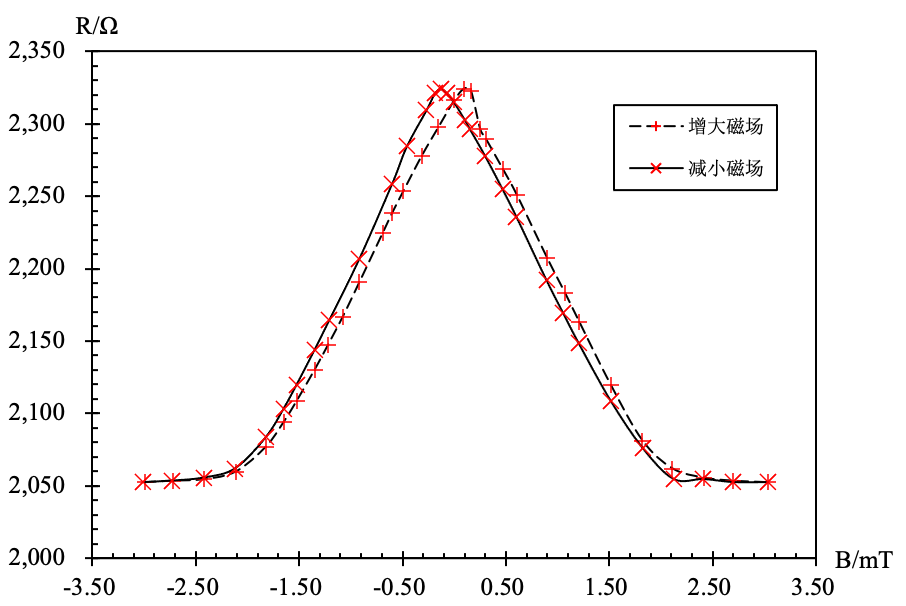
\includegraphics[width=0.9\linewidth]{../Data/GMR-Plot-01-01-excel.png}
    \caption{巨磁电阻元件阻值与外加磁感应强度关系图} \label{fig:magnetoresistance}
\end{figure}

如图\ref{fig:magnetoresistance}所示。可以看出,随着外加磁场的增大,电阻值出现显著下降:在外加磁感应强度接近零时,阻值约为$2324~$\si{\ohm};磁感应强度增大至$H_s \approx 2.0$\si{\milli\tesla}之后,电阻值趋近于$R(H_s)\approx 2050~$\si{\ohm},提示此时磁电阻达到饱和状态;而在达到饱和前,电阻值随磁感应强度有一定变化率,且与外加磁感应强度近似为线性关系。

根据上述测量结果,还可得到$\mathrm{MR_2}$值与外加磁场$B$的关系。其中,$\mathrm{MR_2}$由如下公式定义:

\begin{equation}\label{eq:mr2}
    \mathrm{MR_2} = \frac{R(H) - R(H_s)}{R(H_s)} \times 100\%
\end{equation}

作图如下:
\begin{figure}[H]
    \centering
    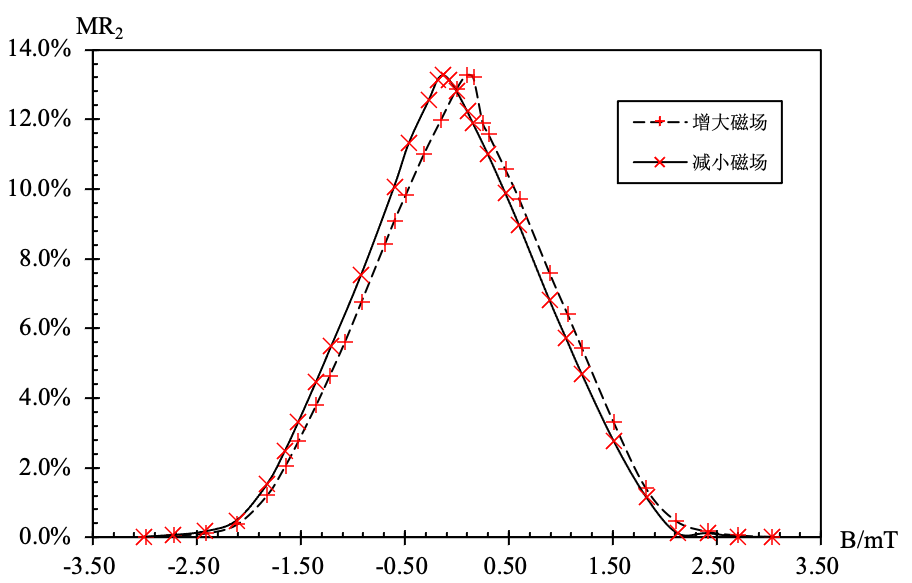
\includegraphics[width=0.9\linewidth]{../Data/GMR-Plot-01-02-excel.png}
    \caption{巨磁电阻变化率$\mathrm{MR_2}$与外加磁感应强度关系图} \label{fig:magnetoresistance}
\end{figure}

值得注意的是,在单向增大磁场和单向减小磁场的过程中,电阻值的变化情况并不完全相同。在增大磁场的过程中,$\mathrm{MR_2}$极大值出现在$B\approx 0.09$ \si{\milli\tesla}处,而在减小磁场的过程中,$\mathrm{MR_2}$值极小值出现在$B\approx -0.13$ \si{\milli\tesla}处,由此验证GMR元件中铁磁层的磁化具有一定滞回特性。

\subsection{GMR模拟传感器的磁电转换特性测量}

在单向增大磁场和单向减小磁场的过程中,测得GMR模拟传感器输出电压$U_s$与外加磁场关系如下图所示:

\begin{figure}[H]
    \centering
    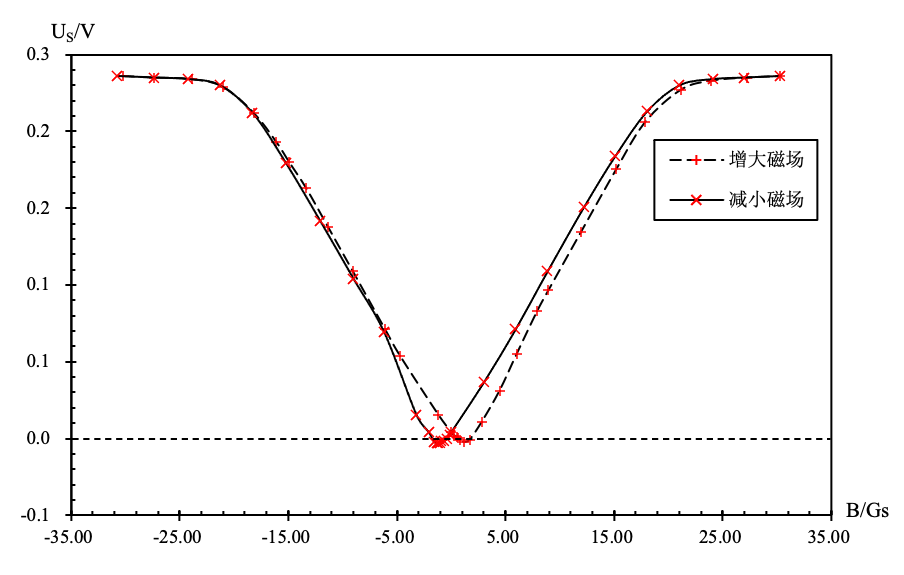
\includegraphics[width=0.9\linewidth]{../Data/GMR-Plot-02-excel.png}
    \caption{GMR模拟传感器磁电转换特性曲线} \label{fig:gmrsensor}
\end{figure}

如图\ref{fig:gmrsensor}所示。可以看出,随着外加磁场的增大,输出电压$U_s$出现显著变化。在外加磁感应强度接近零时,输出电压约为0;磁感应强度增大至约$2.0$\si{\milli\tesla}之后,输出电压达到相对恒定值(约$0.236$\si{\milli\volt}),提示此时GMR模拟传感器达到饱和状态。而在磁感应强度达到饱和值之前,输出电压随磁感应强度有一定变化率,且近似为线性关系。

对比直接测量GMR元件电阻的结果可以看出,GMR模拟传感器的电桥结构使得原先相对变化值约$10\%$的阻值变化被放大为输出电压变化约$0.236$\si{\milli\volt}的信号输出,验证了GMR模拟传感器的有效性。

\subsection{GMR开关(数字)传感器的磁电转换特性测量}

在单向增大磁场和单向减小磁场的过程中,注意到GMR开关传感器的输出电压$U_s$与外加磁场关系表现出显著的“台阶函数”特征。具体地,在单向增大磁场的过程中,测得GMR开关传感器输出电压$U_s$在外加磁场从$-0.8$\si{\milli\tesla}增加至$-0.4$\si{\milli\tesla}附近时,输出电压从$1.928$\si{\volt}跃变至$0.003$\si{\volt},随后在增加磁场至$0.5$/\si{\milli\tesla}附近时,输出电压再次发生跳变,升至$1.928$\si{\volt};而在单向减小磁场的过程中,也可以观察到类似的跳变现象。

为准确确认跳变发生的励磁电流$I_m$,先后多次在励磁电流$I_m$取$-40 ~ \mathrm{mA}$至$40 ~ \mathrm{mA}$范围内,单向增减外加磁场,记录发生高低电平之间发生跃变对应的临界励磁电流。测量结果如下表:

\begin{table}[H]
    \centering
    \captionnamefont{\wuhao\bf\heiti}
    \captiontitlefont{\wuhao\bf\heiti}
    \caption{GMR开关传感器磁电转换特性测量数据} \label{tab:gmr_switch}
    \liuhao
        \begin{tabular}{ccccc}
        \toprule
        \multirow{2}{*}{测量轮次} & \multicolumn{4}{c}{临界励磁电流} $I_m$ /\si{\milli\ampere} \\
        &  \multicolumn{2}{c}{增大磁场} &  \multicolumn{2}{c}{减小磁场}\\
        \midrule
            1 & -13.7 & 18.8 & 13   & -19.7 \\
            2 & -13.8 & 18.6 & 13.4 & -19   \\
            3 &       &      &      & -18.9 \\
        选取值 & -13.8 & 18.6 & 13.4 & -18.9 \\
        \bottomrule
        \end{tabular}
\end{table}

据此,确认增大磁场时,信号电压骤降发生在$-0.416$\si{\milli\tesla}处,信号电压陡增发生在$0.561$\si{\milli\tesla}处;减小磁场时,信号电压骤降发生在$-0.404$\si{\milli\tesla}处,信号电压陡增发生在$0.416$\si{\milli\tesla}处。


\subsection{使用GMR模拟传感器测量电流}

先后在低偏置磁场和适当偏置磁场状态下,单向增大和减小待测导线电流,测得GMR模拟传感器输出电压$U_s$与外加电流关系,分别进行线性拟合以及作图,得到下图以及下表所示拟合结果:

\begin{figure}[H]
    \centering
    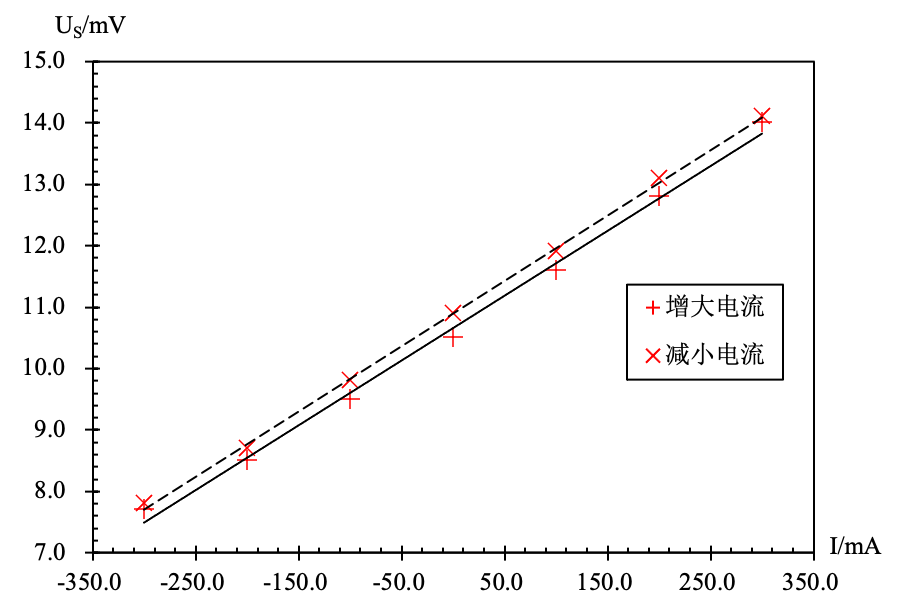
\includegraphics[width=0.9\linewidth]{../Data/GMR-Plot-04-01-excel.png}
    \caption{低偏置磁场下GMR模拟传感器输出电压与导线电流关系图} \label{fig:gmr_current_low}
\end{figure}

\begin{figure}[H]
    \centering
    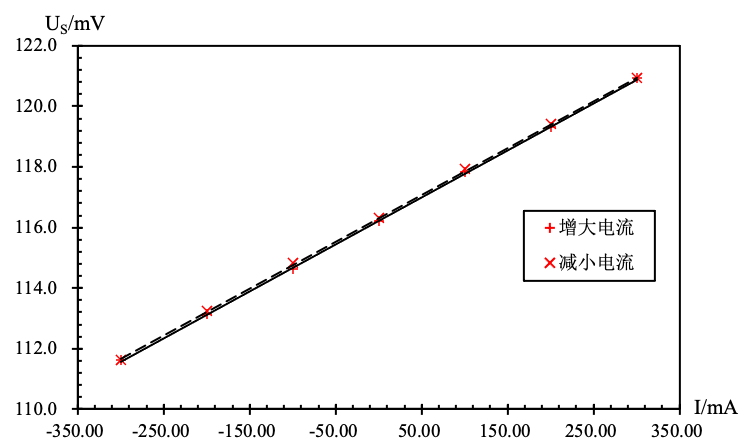
\includegraphics[width=0.9\linewidth]{../Data/GMR-Plot-04-02-excel.png}
    \caption{适当偏置磁场下GMR模拟传感器输出电压与导线电流关系图} \label{fig:gmr_current}
\end{figure}

\begin{table}[H]
    \centering
    \captionnamefont{\wuhao\bf\heiti}
    \captiontitlefont{\wuhao\bf\heiti}
    \caption{GMR模拟传感器测量电流拟合结果} \label{tab:gmr_current_fit}
    \liuhao
    \begin{tabular}{ccccc}
        \toprule
        偏置 & 增大/减 & 斜率 & 截距& 相关系数\\
        磁场 & 小电流 & $k ~ /\mathrm{V\cdot mA^{-1}} $ &$b$/ \si{\milli\volt} &$r^2$ \\
        \midrule
        \multirow{4}{*}{低}   & \multirow{2}{*}{增大} & $0.0106$ & $10.65$ & \multirow{2}{*}{$0.99600$} \\
         & & $\pm 0.0003$ & $\pm 0.06$ & \\
                                  & \multirow{2}{*}{减小} & $0.0106$ & $10.90$ & \multirow{2}{*}{$0.99923$}\\
         & & $\pm 0.0002$ & $\pm 0.03$ & \\
        \multirow{4}{*}{适当} & \multirow{2}{*}{增大} & $0.01553$ & $116.214$ & \multirow{2}{*}{$0.99988$} \\
         & & $\pm 0.00008$ & $\pm 0.015$ & \\
                                  & \multirow{2}{*}{减小} & $0.015500$ & $116.300 $ & \multirow{2}{*}{$0.99985$}\\
         & & $\pm 0.00009$ & $\pm 0.017$ & \\
        \bottomrule
    \end{tabular}
\end{table}

可以看出,在两种偏置磁场状态下,GMR模拟传感器输出电压$U_s$与外加电流$I_s$之间均近似呈线性关系。但在低偏置磁场状态下,前后单向增大电流和单向减小电流的测量结果之间差值较大,提示在低偏置磁场状态下,磁滞现象可能会使得增减电流过程中电流测量值不一致,影响测量精度。除此之外,从$r^2$取值可以看出,低偏置状态下电压与电流关系的线性程度亦不及适当偏置状态下。因而在使用GMR模拟传感器测量电流时,加以适当的偏置磁场有利于提高测量一致性和精度。

\subsection{GMR梯度传感器的特性及应用}

在齿轮转过$0^\circ\~48^\circ$之间的一系列角度过程中,测得GMR梯度传感器输出电压$U_s$与齿轮转过角度关系如下图所示:

\begin{figure}[H]
    \centering
    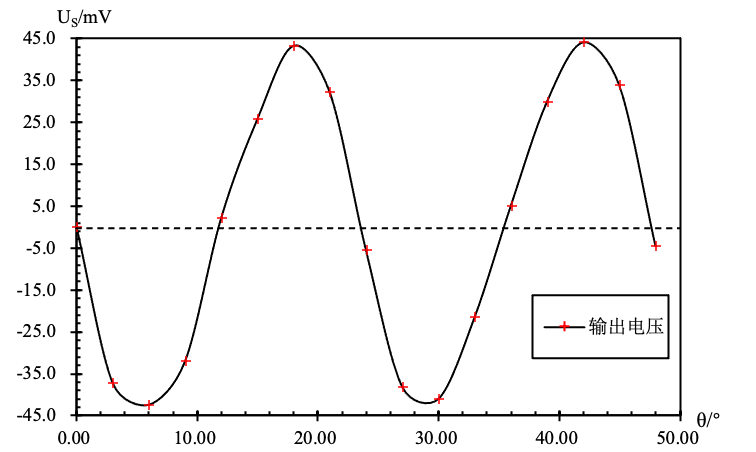
\includegraphics[width=0.9\linewidth]{../Data/GMR-Plot-05-excel.png}
    \caption{GMR梯度传感器特性曲线} \label{fig:gmr_gradient}
\end{figure}

可以看到,齿轮转动过程中GMR梯度传感器输出值$U_s$随齿轮转过角度$\theta$呈现出周期性变化的特征。每一周期对应齿轮转过一个齿,且每个齿对应的角度约为$24^\circ$。在每个齿对应的角度处,输出电压$U_s$出现明显的跃变,且在每个齿对应的角度处,输出电压$U_s$的值近似相同。由此可以验证,GMR梯度传感器可用于角位移测量。

\subsection{磁记录与读出}

本部分实验中在磁卡上写入二进制编码,并在移动磁卡通过读磁头时,记录输出电压$U_s$随磁卡位置变化的关系。测量结果如下表:

\begin{table}[H]
    \centering
    \captionnamefont{\wuhao\bf\heiti}
    \captiontitlefont{\wuhao\bf\heiti}
    \caption{磁记录与读出测量数据} \label{tab:magnetic_record}
    \liuhao
    \begin{tabular}{ccc}
        \toprule
        磁卡位置 & 写入数据& 输出电压 $U_s$/\si{\milli\volt} \\
        \midrule
        1 & 1 & 1.928 \\ 
        2 & 1 & 1.928 \\ 
        3 & 0 & 0.003 \\ 
        4 & 0 & 0.003 \\ 
        5 & 1 & 1.928 \\ 
        6 & 1 & 1.928 \\ 
        7 & 0 & 0.003 \\ 
        8 & 0 & 0.003 \\ 
        \bottomrule
    \end{tabular}
\end{table}

可以看到,在磁卡上写入的二进制编码与读出时输出电压$U_s$之间存在明显的对应关系。每个二进制位对应一个磁条区域,且每个磁条区域对应的输出电压$U_s$近似相同。由此可以验证,磁读写组件可用于磁性记录材料中信息写入以及使用自旋阀器件进行信息读出。

\subsection{自旋阀磁电阻的测量装置与方法}
在单向增大磁场和单向减小磁场的过程中,在初步测量中测得自旋阀器件电阻$R$与外加磁场关系如下表:
\begin{table}[H]
    \centering
    \captionnamefont{\wuhao\bf\heiti}
    \captiontitlefont{\wuhao\bf\heiti}
    \caption{自旋阀磁电阻初步测量数据表} \label{tab:spin_valve}
    \liuhao
    \begin{tabular}{ccccc}
        \toprule
        励磁电流& 磁感应强度 & 自旋阀器件电流 & 电压 & 电阻 \\
        $I_m$/\si{\milli\ampere} & $B/$\si{\milli\tesla} & $I_s$ / \si{\micro\ampere} & $U_s$/\si{\milli\volt} & $R/$\si{\milli\ohm} \\
        \midrule
        1.0 & 3.8560 & 3.910 & 0.972 & 4023 \\ 
        0.9 & 3.4704 & 3.955 & 0.983 & 4023 \\ 
        0.8 & 3.0848 & 3.954 & 0.983 & 4022 \\ 
        0.7 & 2.6992 & 3.940 & 0.978 & 4029 \\ 
        0.6 & 2.3136 & 3.930 & 0.978 & 4018 \\ 
        0.5 & 1.9280 & 3.950 & 0.981 & 4027 \\ 
        0.4 & 1.5424 & 3.950 & 0.981 & 4027 \\ 
        0.3 & 1.1568 & 3.946 & 0.977 & 4039 \\ 
        0.2 & 0.7712 & 3.946 & 0.970 & 4068 \\ 
        0.1 & 0.3856 & 3.943 & 0.969 & 4069 \\ 
        0.0 & 0.0000 & 3.944 & 0.969 & 4070 \\
        \bottomrule
    \end{tabular}
\end{table}

在实际测量中,发现电流表测量值整体变化趋势并不显著而伴有较显著的随时间漂移,难以进行准确读数;推断原因为电源输出电压不稳定。经指导教师同意,放弃本部分实验。

\section{结论}
用准确、精炼的语言归纳总结使用的方法以及研究结果。

说明研究的创新价值和应用价值,包括对科技工作者的研究的价值和对产业发展的价值。

可说明自己做本实验的总结、收获和体会,对实验中发现的问题提出自己的建议。


%%%%%%%%%%%%%%%%%%%%%%%%%%%%%%%%%%%%%%%%%%%%%%%%%%%%%%%%%%%%%%%%
%  参考文献
%%%%%%%%%%%%%%%%%%%%%%%%%%%%%%%%%%%%%%%%%%%%%%%%%%%%%%%%%%%%%%%%
%  参考文献按GB/T 7714-2015《文后参考文献著录规则》的要求著录. 
%  参考文献在正文中的引用方法:\cite{bib文件条目的第一行}

\renewcommand\refname{\heiti\wuhao\centerline{参考文献}\global\def\refname{参考文献}}
\vskip 12pt


\let\OLDthebibliography\thebibliography
\renewcommand\thebibliography[1]{
  \OLDthebibliography{#1}
  \setlength{\parskip}{0pt}
  \setlength{\itemsep}{0pt plus 0.3ex}
}

{
\renewcommand{\baselinestretch}{0.9}
\liuhao
\bibliographystyle{gbt7714-numerical}
\bibliography{./Report/TempExample}
}

\appendix
\section{部分实验数据}

\begin{table}[H]
    \centering
    \captionnamefont{\wuhao\bf\heiti}
    \captiontitlefont{\wuhao\bf\heiti}
    \caption{增大磁感应强度过程中巨磁阻特性测量数据} \label{tab:magnetoresistance_incr}
    \liuhao
    \begin{tabular}{ccccc}
        \toprule
        励磁电流 & 磁感应强度 & GMR器件电流 & 电阻 & \multirow{2}{*}{$\mathrm{MR_2}$}\\
        $I_m$/\si{\milli\ampere} & $B$ /\si{\milli\tesla} & $I_R$$ /\si{\milli\ampere}$ & $R$$/\si{\ohm} $& \\
        \midrule
        -99.1  & -2.99 & 1.949 & 2052 & 0.02\%  \\
        -90.3  & -2.72 & 1.948 & 2053 & 0.07\%  \\
        -80.1  & -2.42 & 1.947 & 2054 & 0.12\%  \\
        -70.0  & -2.11 & 1.942 & 2060 & 0.38\%  \\
        -60.4  & -1.82 & 1.926 & 2077 & 1.21\%  \\
        -54.6  & -1.65 & 1.910 & 2094 & 2.06\%  \\
        -50.5  & -1.52 & 1.897 & 2109 & 2.76\%  \\
        -44.8  & -1.35 & 1.878 & 2130 & 3.80\%  \\
        -40.5  & -1.22 & 1.863 & 2147 & 4.63\%  \\
        -35.7  & -1.08 & 1.846 & 2167 & 5.60\%  \\
        -30.4  & -0.92 & 1.826 & 2191 & 6.75\%  \\
        -22.9  & -0.69 & 1.798 & 2225 & 8.42\%  \\
        -19.9  & -0.60 & 1.787 & 2238 & 9.08\%  \\
        -16.3  & -0.49 & 1.775 & 2254 & 9.82\%  \\
        -10.4  & -0.31 & 1.756 & 2278 & 11.01\% \\
        -5.1   & -0.15 & 1.741 & 2298 & 11.97\% \\
        0.0    & 0.00  & 1.727 & 2316 & 12.87\% \\
        3.1    & 0.09  & 1.721 & 2324 & 13.27\% \\
        5.3    & 0.16  & 1.722 & 2323 & 13.20\% \\
        8.3    & 0.25  & 1.742 & 2296 & 11.90\% \\
        10.1   & 0.30  & 1.747 & 2290 & 11.58\% \\
        15.5   & 0.47  & 1.763 & 2269 & 10.57\% \\
        20.0   & 0.60  & 1.777 & 2251 & 9.70\%  \\
        29.7   & 0.90  & 1.812 & 2208 & 7.58\%  \\
        35.4   & 1.07  & 1.832 & 2183 & 6.40\%  \\
        40.0   & 1.21  & 1.849 & 2163 & 5.43\%  \\
        50.1   & 1.51  & 1.887 & 2120 & 3.30\%  \\
        60.3   & 1.82  & 1.922 & 2081 & 1.42\%  \\
        69.9   & 2.11  & 1.940 & 2062 & 0.48\%  \\
        80.0   & 2.41  & 1.946 & 2055 & 0.17\%  \\
        89.4   & 2.70  & 1.948 & 2053 & 0.07\%  \\
        100.5  & 3.03  & 1.949 & 2052 & 0.02\%  \\
        \bottomrule
    \end{tabular}
\end{table}

\begin{table}[H]
    \centering
    \captionnamefont{\wuhao\bf\heiti}
    \captiontitlefont{\wuhao\bf\heiti}
    \caption{减小磁感应强度过程中巨磁阻特性测量数据} \label{tab:magnetoresistance_desc}
    \liuhao
    \begin{tabular}{ccccc}
        \toprule
        励磁电流 & 磁感应强度 & GMR器件电流 & 电阻 & \multirow{2}{*}{$\mathrm{MR_2}$}\\
        $I_m$/\si{\milli\ampere} & $B$ /\si{\milli\tesla} & $I_R$$ /\si{\milli\ampere}$ & $R$$/\si{\ohm} $& \\
        \midrule
        -99.7 & -3.01 & 1.949 & 2052 &  0.02\%  \\
        -90.4 & -2.73 & 1.948 & 2053 &  0.07\%  \\
        -80.2 & -2.42 & 1.946 & 2055 &  0.17\%  \\
        -70.2 & -2.12 & 1.940 & 2062 &  0.48\%  \\
        -60.4 & -1.82 & 1.920 & 2083 &  1.53\%  \\
        -54.7 & -1.65 & 1.902 & 2103 &  2.49\%  \\
        -50.5 & -1.52 & 1.887 & 2120 &  3.30\%  \\
        -44.8 & -1.35 & 1.866 & 2144 &  4.47\%  \\
        -40.0 & -1.21 & 1.848 & 2165 &  5.48\%  \\
        -30.5 & -0.92 & 1.813 & 2206 &  7.52\%  \\
        -19.9 & -0.60 & 1.771 & 2259 & 10.07\%  \\
        -15.2 & -0.46 & 1.751 & 2284 & 11.33\%  \\
        -8.9  & -0.27 & 1.732 & 2309 & 12.55\%  \\
        -6.1  & -0.18 & 1.723 & 2322 & 13.14\%  \\
        -4.3  & -0.13 & 1.721 & 2324 & 13.27\%  \\
        -2.4  & -0.07 & 1.723 & 2322 & 13.14\%  \\
        0.0   & 0.00  & 1.728 & 2315 & 12.81\%  \\
        3.4   & 0.10  & 1.737 & 2303 & 12.22\%  \\
        5.1   & 0.15  & 1.742 & 2296 & 11.90\%  \\
        9.9   & 0.30  & 1.756 & 2278 & 11.01\%  \\
        15.5  & 0.47  & 1.774 & 2255 &  9.88\%  \\
        19.9  & 0.60  & 1.789 & 2236 &  8.96\%  \\
        29.6  & 0.89  & 1.825 & 2192 &  6.81\%  \\
        34.9  & 1.05  & 1.844 & 2169 &  5.71\%  \\
        39.9  & 1.20  & 1.862 & 2148 &  4.69\%  \\
        50.1  & 1.51  & 1.897 & 2109 &  2.76\%  \\
        60.4  & 1.82  & 1.927 & 2076 &  1.16\%  \\
        70.3  & 2.12  & 1.947 & 2054 &  0.12\%  \\
        79.9  & 2.41  & 1.947 & 2054 &  0.12\%  \\
        89.4  & 2.70  & 1.949 & 2052 &  0.02\%  \\
        100.5 & 3.03  & 1.949 & 2052 &  0.02\%  \\
        \bottomrule
    \end{tabular}
\end{table}



\begin{table}[H]
    \centering
    \captionnamefont{\wuhao\bf\heiti}
    \captiontitlefont{\wuhao\bf\heiti}
    \caption{增大磁场过程中GMR模拟传感器磁电转换特性测量数据} \label{tab:gmrsenso_incr}
    \liuhao
    \begin{tabular}{ccc}
        \toprule
        励磁电流 & 磁感应强度 & 输出电压  \\
        $I_m$/\si{\milli\ampere} & $B$/\si{\milli\tesla} & $U_s$/\si{\milli\volt} \\
        \midrule
        -100.0 & -3.02 & 0.236    \\
        -90.6  & -2.73 & 0.235    \\
        -79.1  & -2.39 & 0.234    \\
        -69.6  & -2.10 & 0.229    \\
        -60.2  & -1.82 & 0.212    \\
        -53.3  & -1.61 & 0.193    \\
        -49.4  & -1.49 & 0.180    \\
        -44.2  & -1.33 & 0.163    \\
        -37.6  & -1.13 & 0.138    \\
        -30.0  & -0.90 & 0.109    \\
        -20.1  & -0.61 & 0.0710   \\
        -15.5  & -0.47 & 0.0536   \\
        -3.9   & -0.12 & 0.0155   \\
        0.0    & 0.00  & 0.0042   \\
        0.9    & 0.03  & 0.0019   \\
        1.9    & 0.06  & 0.0008   \\
        2.1    & 0.06  & 0.0003   \\
        2.8    & 0.08  & -0.0011  \\
        4.0    & 0.12  & -0.0025  \\
        5.7    & 0.17  & -0.0011  \\
        9.5    & 0.29  & 0.0109   \\
        14.9   & 0.45  & 0.0311   \\
        20.1   & 0.61  & 0.0549   \\
        26.4   & 0.80  & 0.0830   \\
        29.8   & 0.90  & 0.0964   \\
        39.7   & 1.20  & 0.1342   \\
        50.5   & 1.52  & 0.1752   \\
        59.3   & 1.79  & 0.206    \\
        70.2   & 2.12  & 0.227    \\
        79.5   & 2.40  & 0.233    \\
        90.5   & 2.73  & 0.235    \\
        100.6  & 3.03  & 0.236    \\
        \bottomrule
    \end{tabular}
\end{table}

\begin{table}[H]
    \centering
    \captionnamefont{\wuhao\bf\heiti}
    \captiontitlefont{\wuhao\bf\heiti}
    \caption{减小磁场过程中GMR模拟传感器磁电转换特性测量数据} \label{tab:gmrsensor_desc}
    \liuhao
    \begin{tabular}{ccc}
        \toprule
        励磁电流 & 磁感应强度 & 输出电压  \\
        $I_m$/\si{\milli\ampere} & $B$/\si{\milli\tesla} & $U_s$/\si{\milli\volt} \\
        \midrule
        100.5  & 0.236    &  3.03 \\
        89.6   & 0.235    &  2.70 \\
        80.0   & 0.234    &  2.41 \\
        69.8   & 0.230    &  2.11 \\
        59.9   & 0.213    &  1.81 \\
        50.2   & 0.184    &  1.51 \\
        40.7   & 0.151    &  1.23 \\
        29.5   & 0.1089   &  0.89 \\
        19.7   & 0.0710   &  0.59 \\
        10.0   & 0.0365   &  0.30 \\
        0.0    & 0.0040   &  0.00 \\
        -0.4   & 0.0025   & -0.01 \\
        -1.3   & -0.0004  & -0.04 \\
        -2.2   & -0.0016  & -0.07 \\
        -3.1   & -0.0016  & -0.09 \\
        -3.4   & -0.0026  & -0.10 \\
        -3.8   & -0.0027  & -0.11 \\
        -4.3   & -0.0027  & -0.13 \\
        -5.2   & -0.0020  & -0.16 \\
        -6.8   & 0.0042   & -0.21 \\
        -10.5  & 0.0151   & -0.32 \\
        -20.4  & 0.0691   & -0.62 \\
        -29.8  & 0.1041   & -0.90 \\
        -39.9  & 0.1415   & -1.20 \\
        -50.4  & 0.1793   & -1.52 \\
        -60.6  & 0.212    & -1.83 \\
        -70.6  & 0.230    & -2.13 \\
        -80.1  & 0.234    & -2.42 \\
        -90.5  & 0.235    & -2.73 \\
        -101.9 & 0.236    & -3.07 \\
        \bottomrule
    \end{tabular}
\end{table}

\begin{table}[H]
    \centering
    \captionnamefont{\wuhao\bf\heiti}
    \captiontitlefont{\wuhao\bf\heiti}
    \caption{GMR模拟传感器测量电流数据} \label{tab:gmr_current_low}
    \liuhao
    \begin{tabular}{ccccc}
        \toprule
        \multirow{3}{*}{\makecell[c]{励磁电流 \\ $I_m$/\si{\milli\ampere}}} 
            & \multicolumn{4}{c}{输出电压$U_s$/\si{\milli\volt}} \\
        \cline{2-5}
            & \multicolumn{2}{c}{低偏置磁场} & \multicolumn{2}{c}{适当偏置磁场} \\
        \cline{2-5}
            & 增大电流 & 减小电流 & 增大电流 & 减小电流 \\
        \midrule
        300  & 0.014  &  0.0141 & 0.1209 & 0.1209 \\
        200  & 0.0128 &  0.0131 & 0.1193 & 0.1194 \\
        100  & 0.0116 &  0.0119 & 0.1178 & 0.1179 \\
        0    & 0.0105 &  0.0109 & 0.1162 & 0.1163 \\
        -100 & 0.0095 &  0.0098 & 0.1146 & 0.1148 \\
        -200 & 0.0085 &  0.0087 & 0.1131 & 0.1132 \\
        -300 & 0.0077 &  0.0078 & 0.1116 & 0.1116 \\
        \bottomrule
    \end{tabular}
\end{table}


\begin{table}[H]
    \centering
    \captionnamefont{\wuhao\bf\heiti}
    \captiontitlefont{\wuhao\bf\heiti}
    \caption{GMR梯度传感器特性测量数据} \label{tab:gmr_gradient}
    \liuhao
    \begin{tabular}{ccc}
        \toprule
        齿轮转过角度 $\theta/\mathrm{^\circ}$ & 输出电压 $U_s$/\si{\milli\volt} \\
        \midrule
        0 & 0.0   \\
        3 & -37.3 \\
        6 & -42.5 \\
        9 & -32.1 \\
       12 & 2.2   \\
       15 & 25.8  \\
       18 & 43.3  \\
       21 & 32.1  \\
       24 & -5.6  \\
       27 & -38.2 \\
       30 & -41.1 \\
       33 & -21.6 \\
       36 & 5.0   \\
       39 & 29.9  \\
       42 & 44.1  \\
       45 & 33.8  \\
       48 & -4.6  \\
        \bottomrule
    \end{tabular}
\end{table}


\end{document}
